\section{Project description}

\subsection{Introduction}

The main idea of this project is to develop a waveform generator instrument using an STM32 microcontroller and its built-in DAC. The project has 2 parts:
\begin{itemize}
      \item \textbf{Software}: The application needs to showcase the STM32 capability to output
            waveforms  at sample rates of 100kHz or greater. The software has to include a
            peripheral driver to access the built in DAC using DMA.
      \item \textbf{Hardware}: The device has to to implement a waveform generator output stage
            circuitry that allows to extend the capabilities of the built in DAC.
\end{itemize}

To achieve this goals a custom board was designed and software drivers were developed for the DAC and DMA.

The final product also includes a text interface where the user can setup an arbitrary waveform and the device parses the user input using Flex and Bison.

\begin{figure}[h]
      \captionsetup[subfigure]{labelformat=empty}
      \centering
      \begin{subfigure}[b]{0.45\textwidth}
            \centering
            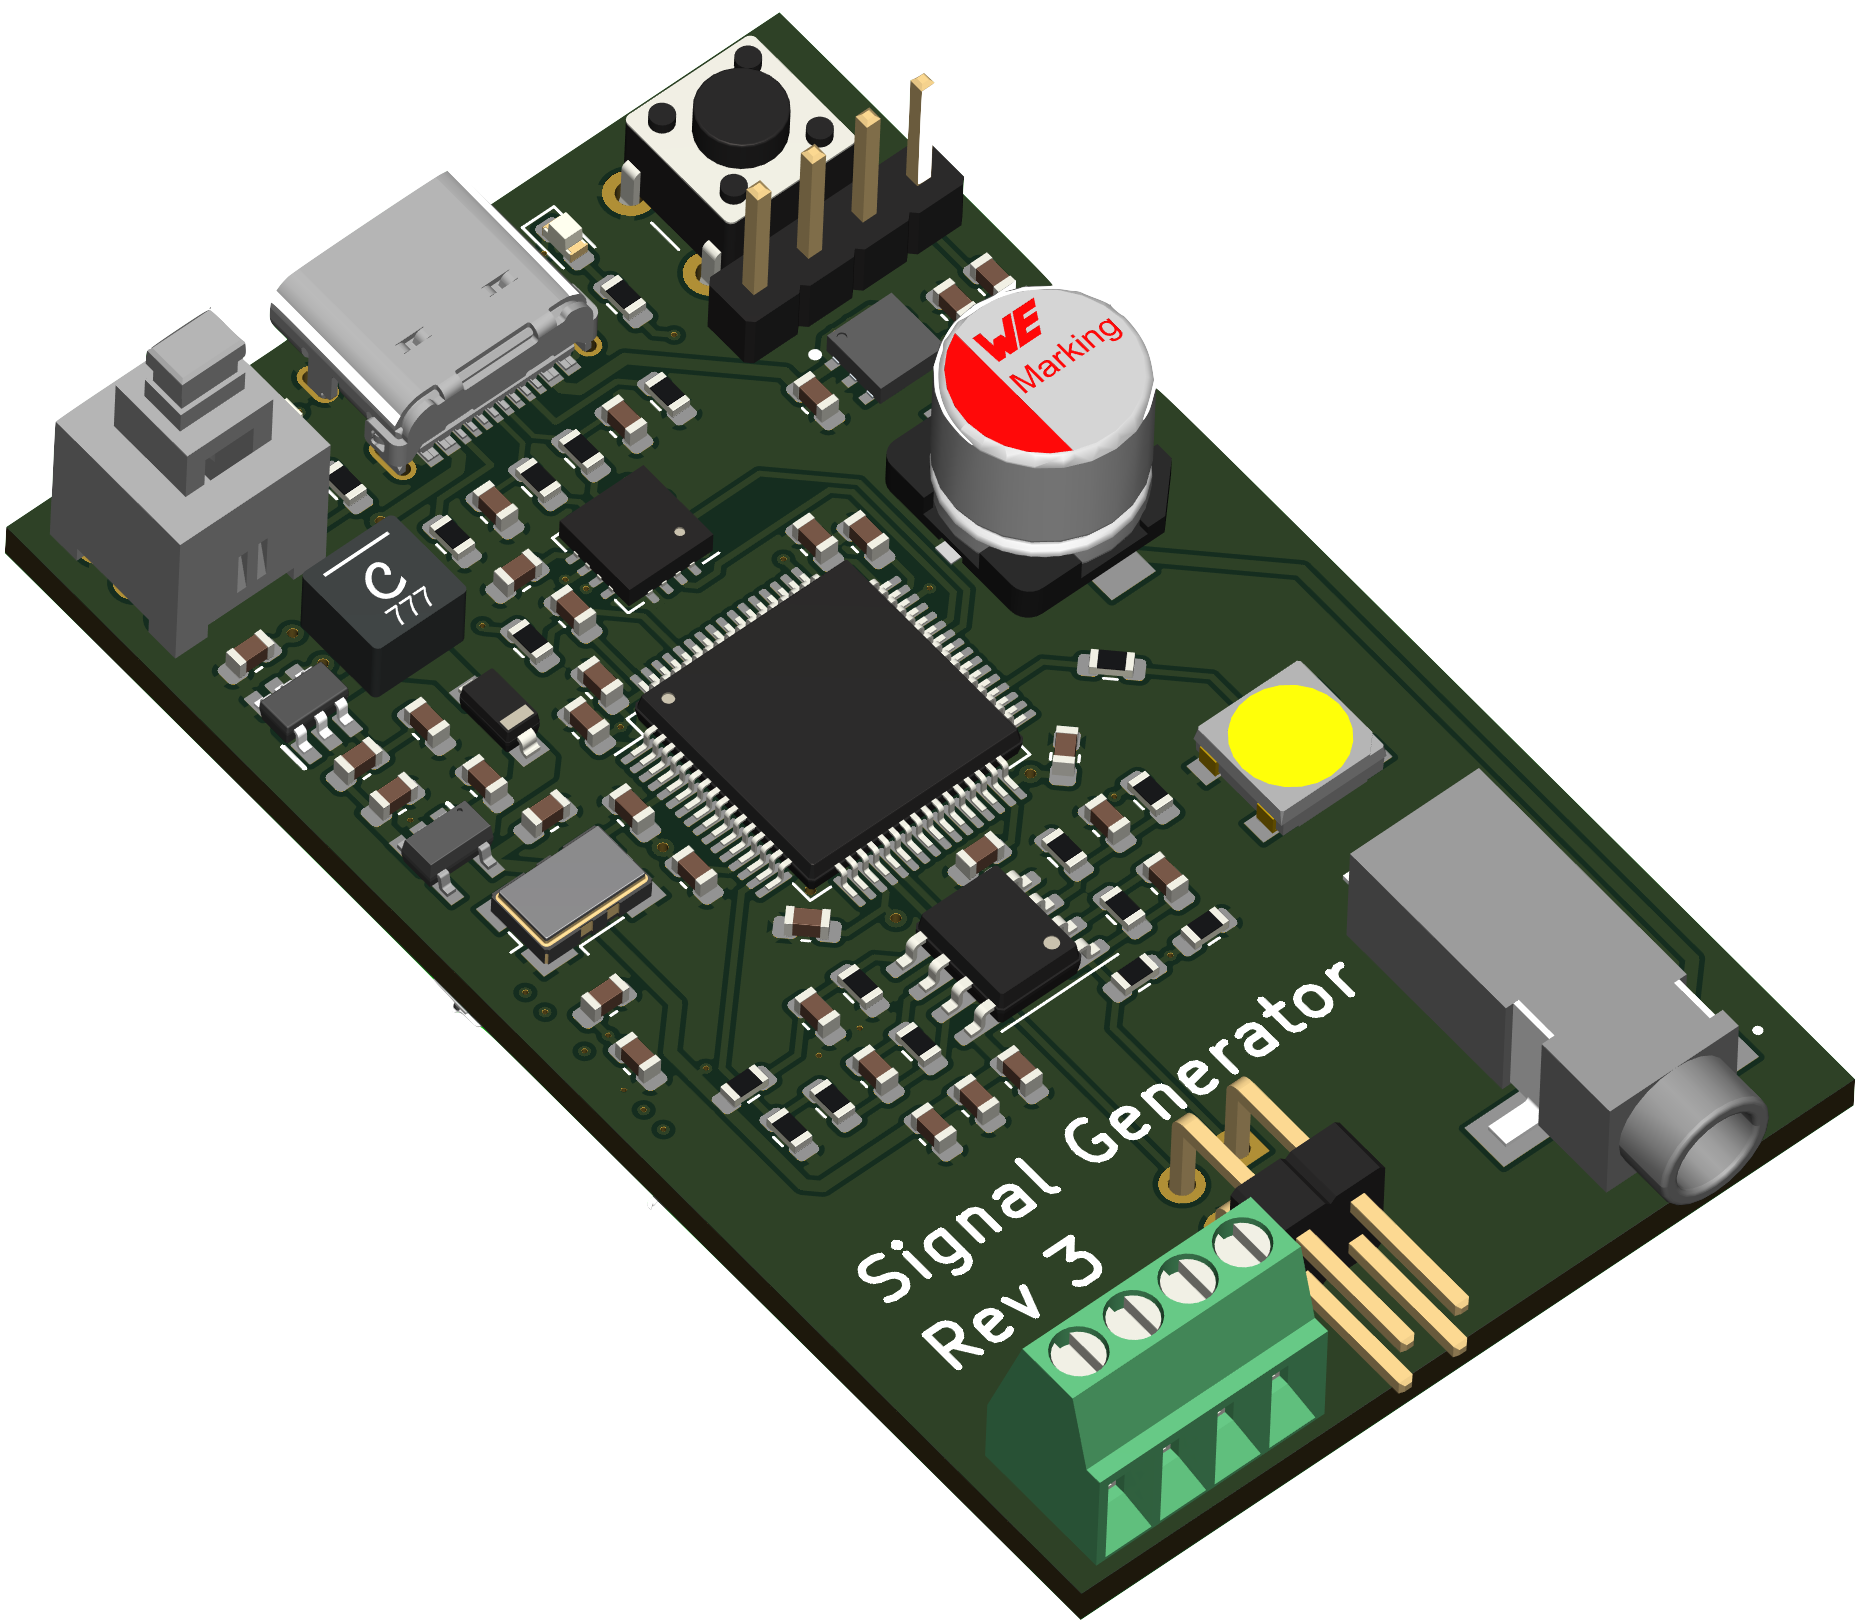
\includegraphics[width=\textwidth]{graphics/pcb_render.png}
            \caption{PCB}
      \end{subfigure}
      \hfill
      \begin{subfigure}[b]{0.50\textwidth}
            \centering
            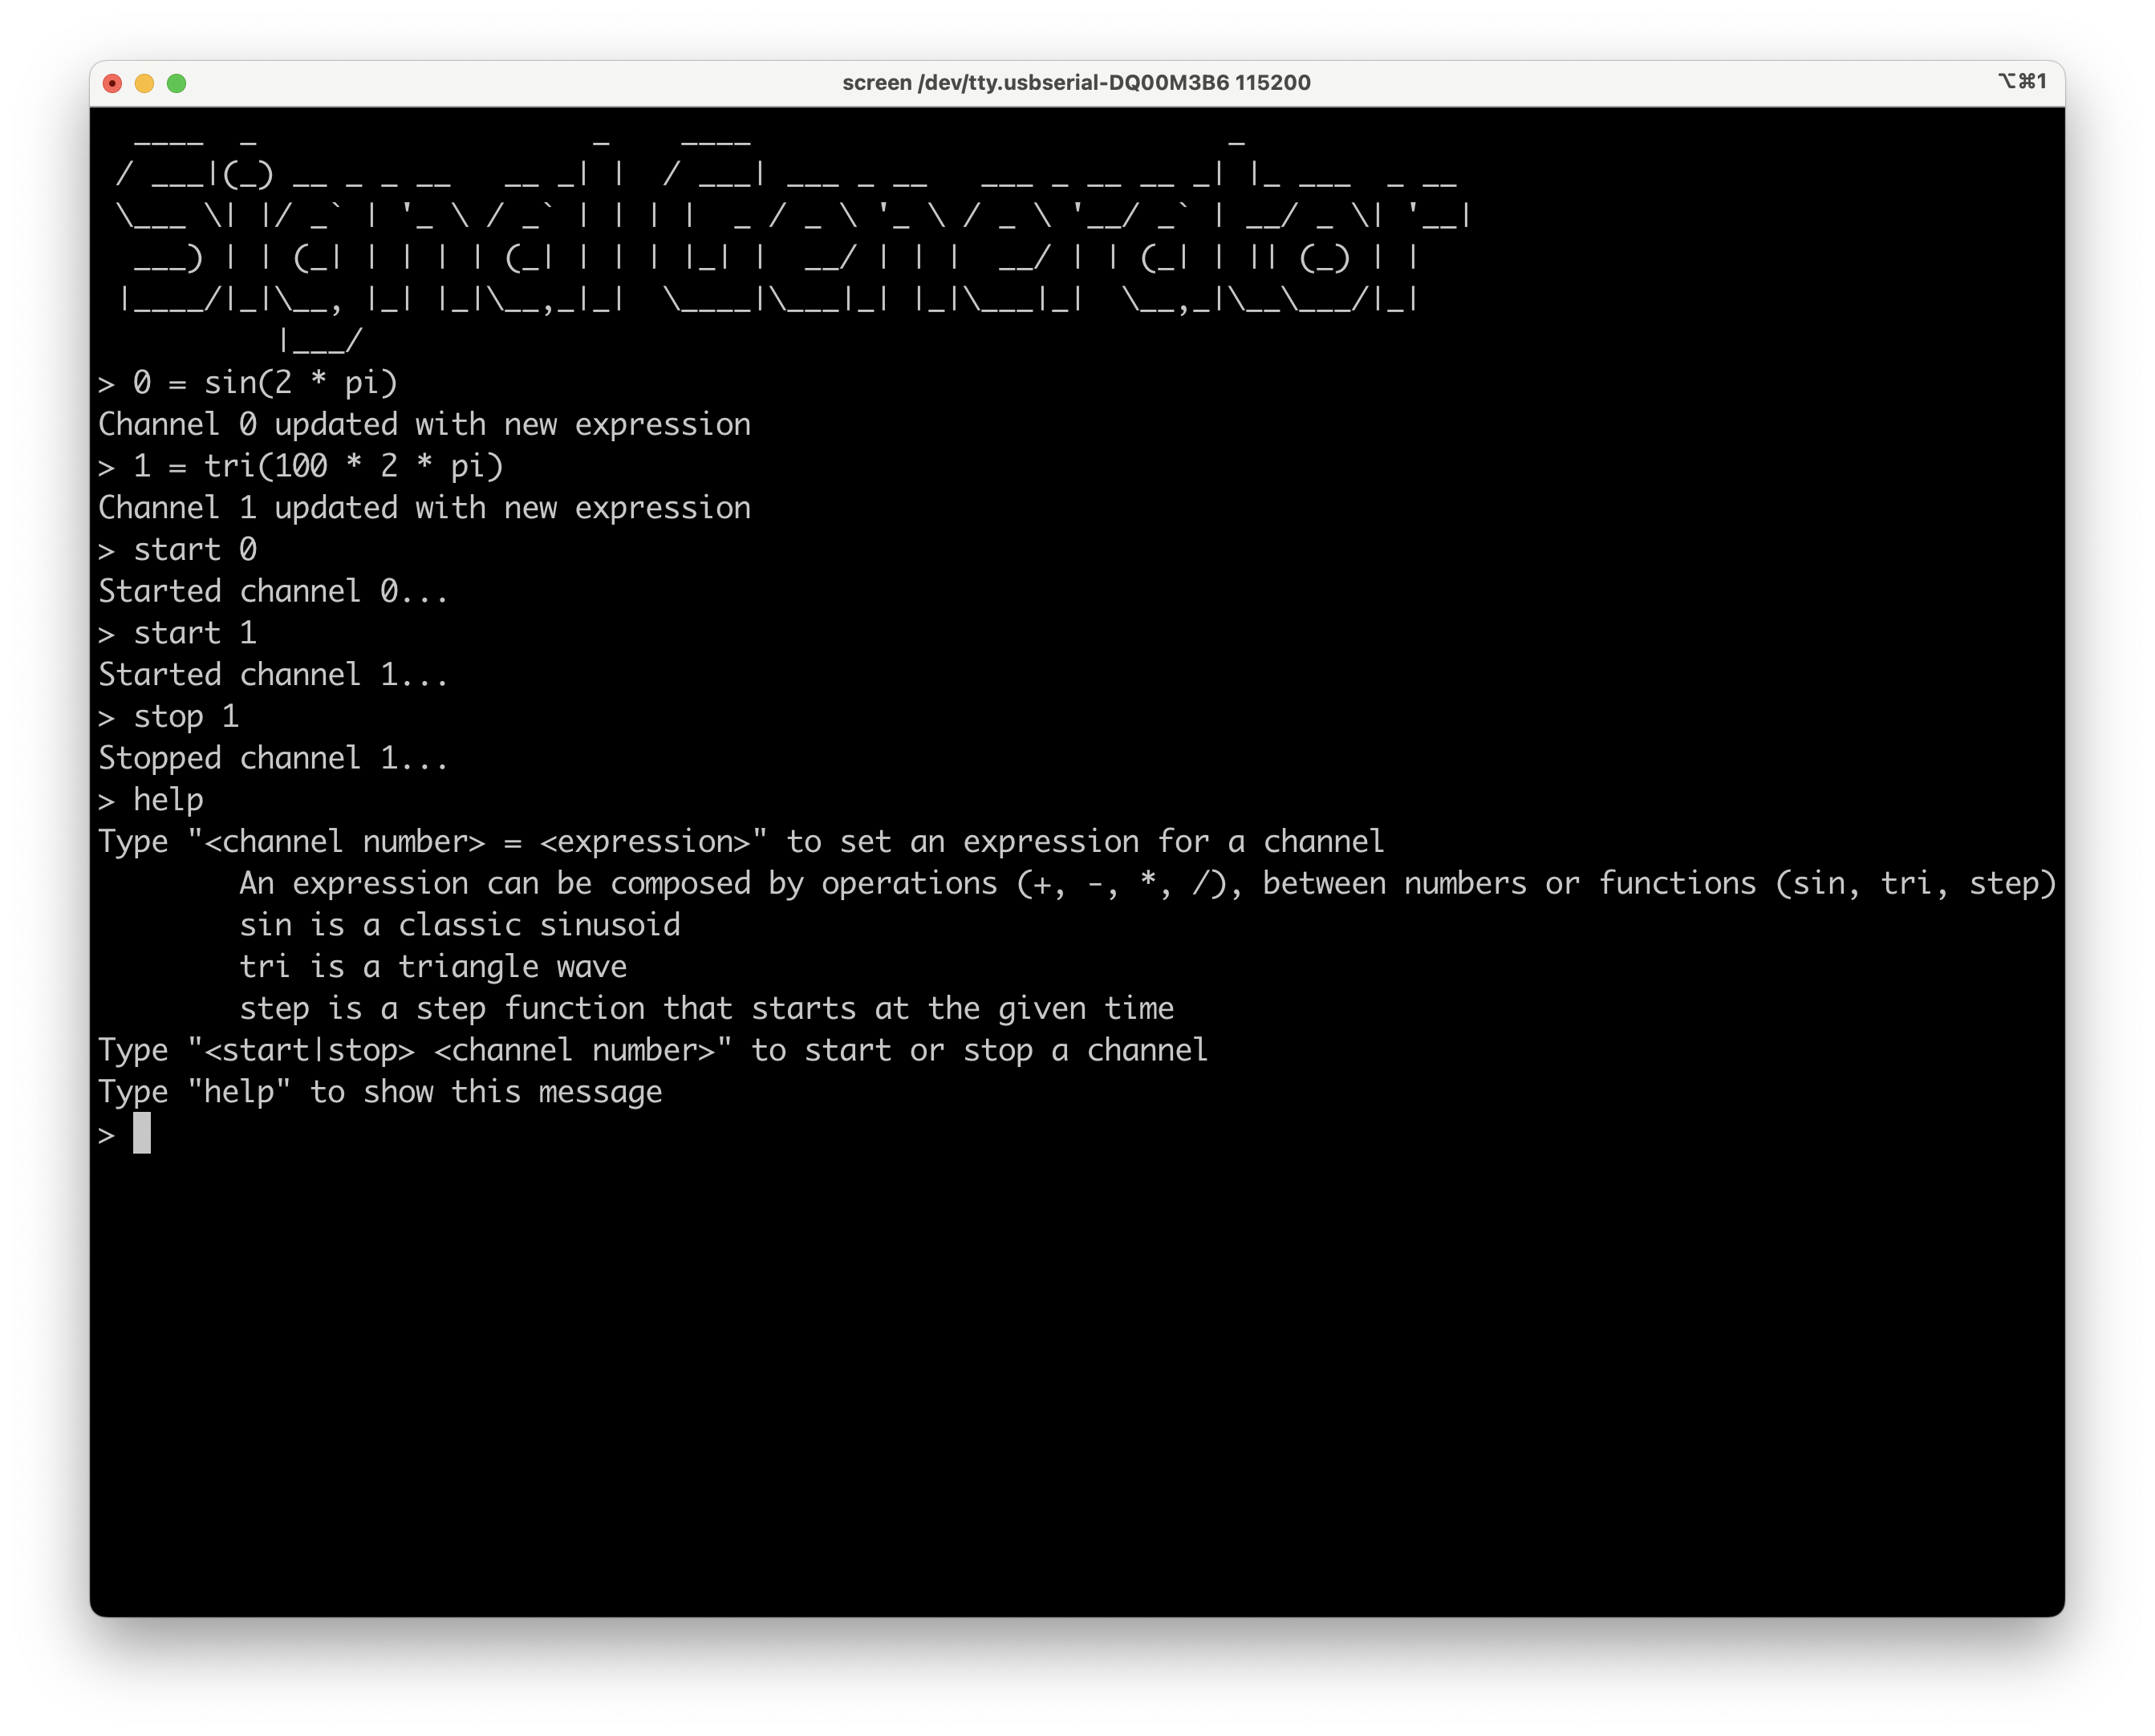
\includegraphics[width=\textwidth]{graphics/console_example.png}
            \caption{Text interface}
      \end{subfigure}
\end{figure}

\subsection{Design of the Printed Circuit Board}

The goal I set out to achieve is create a stand-alone PCB with builtin micro controller and front-end circuit that blends the stm32's built-in features and external components, to produce a high-frequency arbitrary waveforms with a 12V peak without external power supplies.

\subsubsection{Analog Front End}

The stm32 incorporates a Digital-to-Analog Converter (DAC) with an integrated output buffer. When enabled, the buffer allows the DAC to drive external loads directly. However, this comes at the cost of limited driving capability, especially when interfacing with capacitive loads. Disabling the buffer offers a pure analog output, but necessitates an external buffer or amplifier to drive any meaningful external load. The inherent impedance of the DAC's output pin can also cause distortions and constrain the signal's frequency, particularly when dealing with capacitive loads.

\bigbreak

Integrating an external operational amplifier (op-amp) into the analog front-end offers multiple advantages:
\begin{itemize}
      \item  \textbf{Buffering DAC Output}: The op-amp serves as a buffer, isolating the DAC from the actual load. This setup minimizes the effects of the DAC output pin's impedance, enabling the DAC to operate in a near-ideal environment.
      \item \textbf{Voltage Scaling}: Configured in a non-inverting amplifier mode, the op-amp provides adjustable gain, facilitating flexible signal amplitude adjustments.
\end{itemize}

Given that the board is powered via USB, which typically provides 5V, there's a need to step up this voltage to achieve the 12V requirement for the analog front end:
\begin{itemize}
      \item \textbf{Boost Converter}: The TLV61048 boost converter is employed to step up the USB's 5V to 13.12V.
      \item \textbf{Linear Voltage Regulator}: Following the boost converter, an LDO is used to convert the 13.12V from the boost converter to a stable 12V output. This stable 12V supply is crucial to ensure that the analog front-end, especially the operational amplifier, operates with consistency.
\end{itemize}

The opamp circuit also features a voltage divider to feedback the output signal to the STM32's ADC. This could allow the microcontroller to perform automatic calibration of the opamp gains.

\begin{figure}[h]
      \captionsetup[subfigure]{labelformat=empty}
      \centering
      \begin{subfigure}[b]{0.4\textwidth}
            \centering
            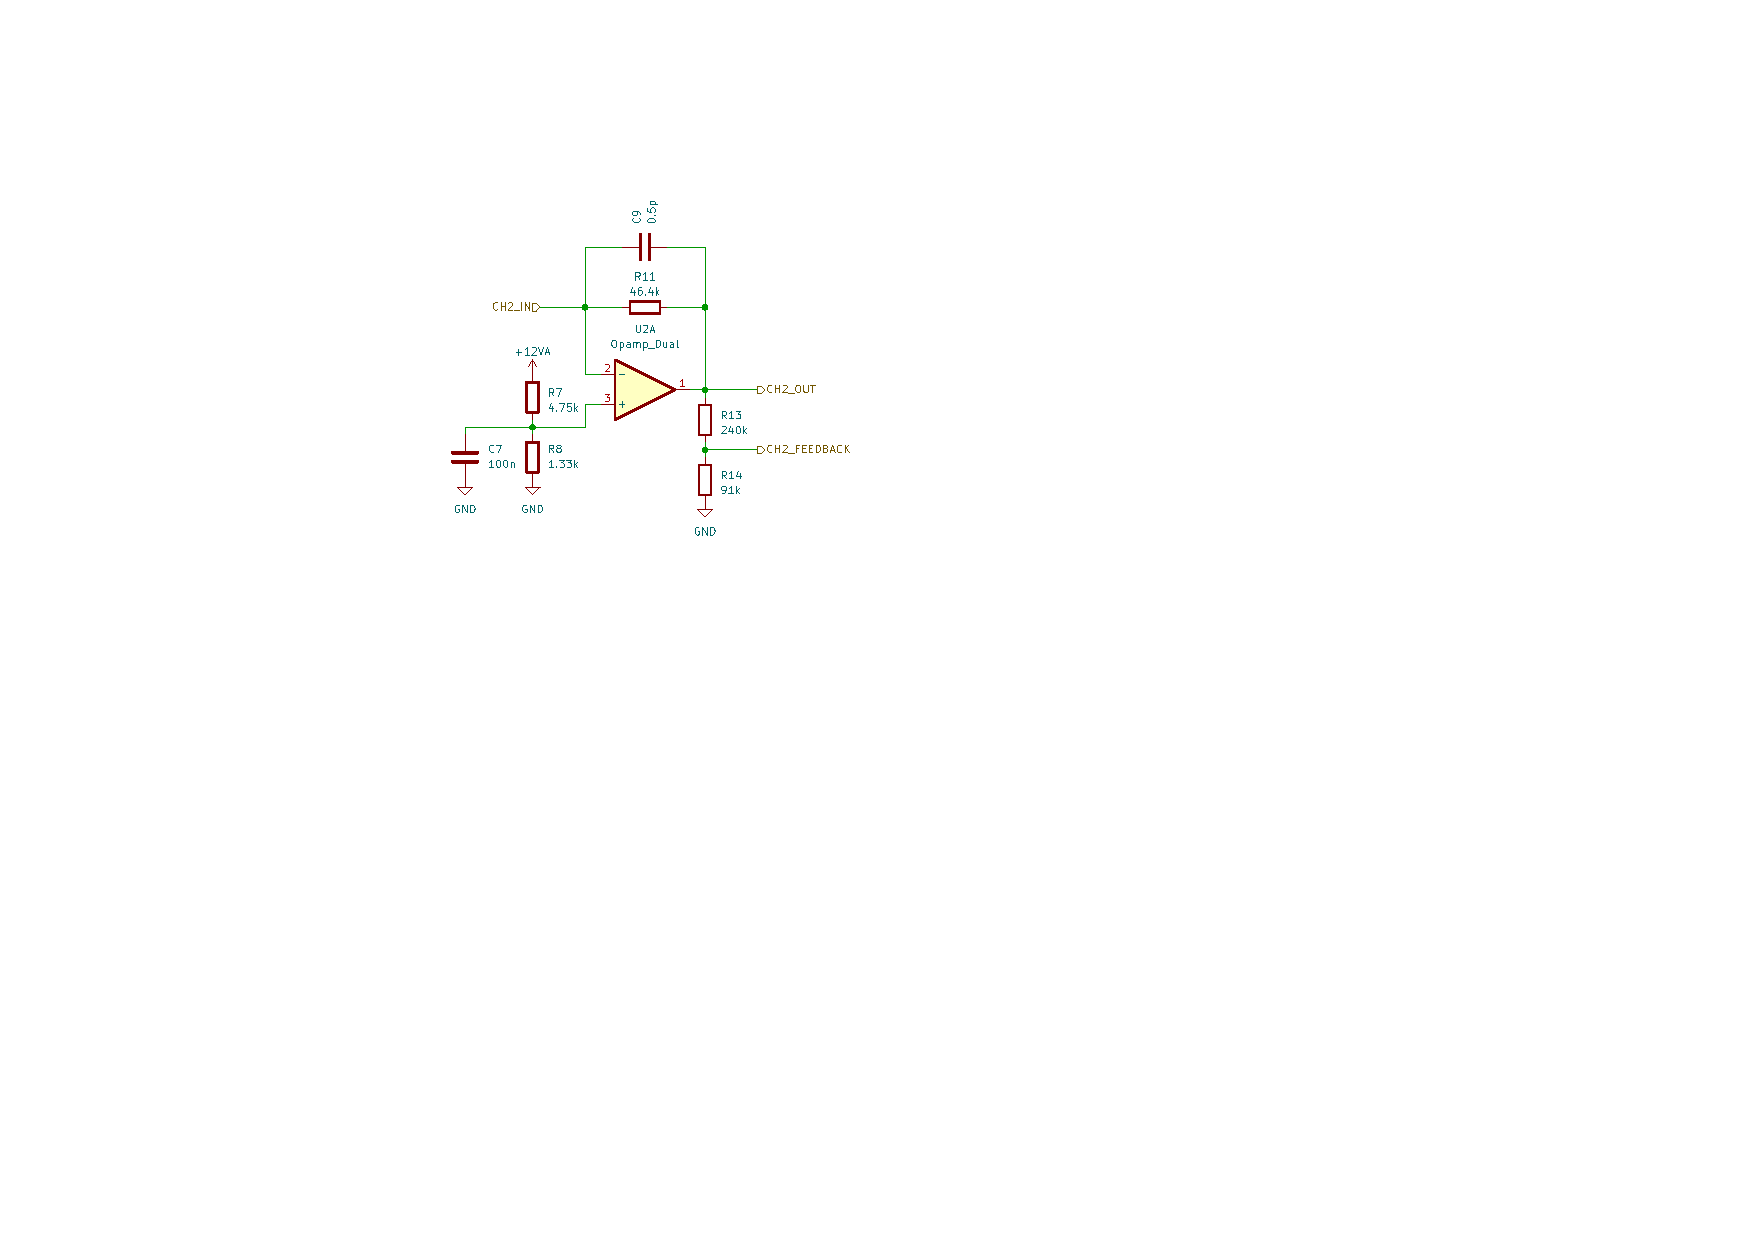
\includegraphics[width=\textwidth]{graphics/front_end.pdf}
            \caption{Front end}
      \end{subfigure}
      \hfill
      \begin{subfigure}[b]{0.59\textwidth}
            \centering
            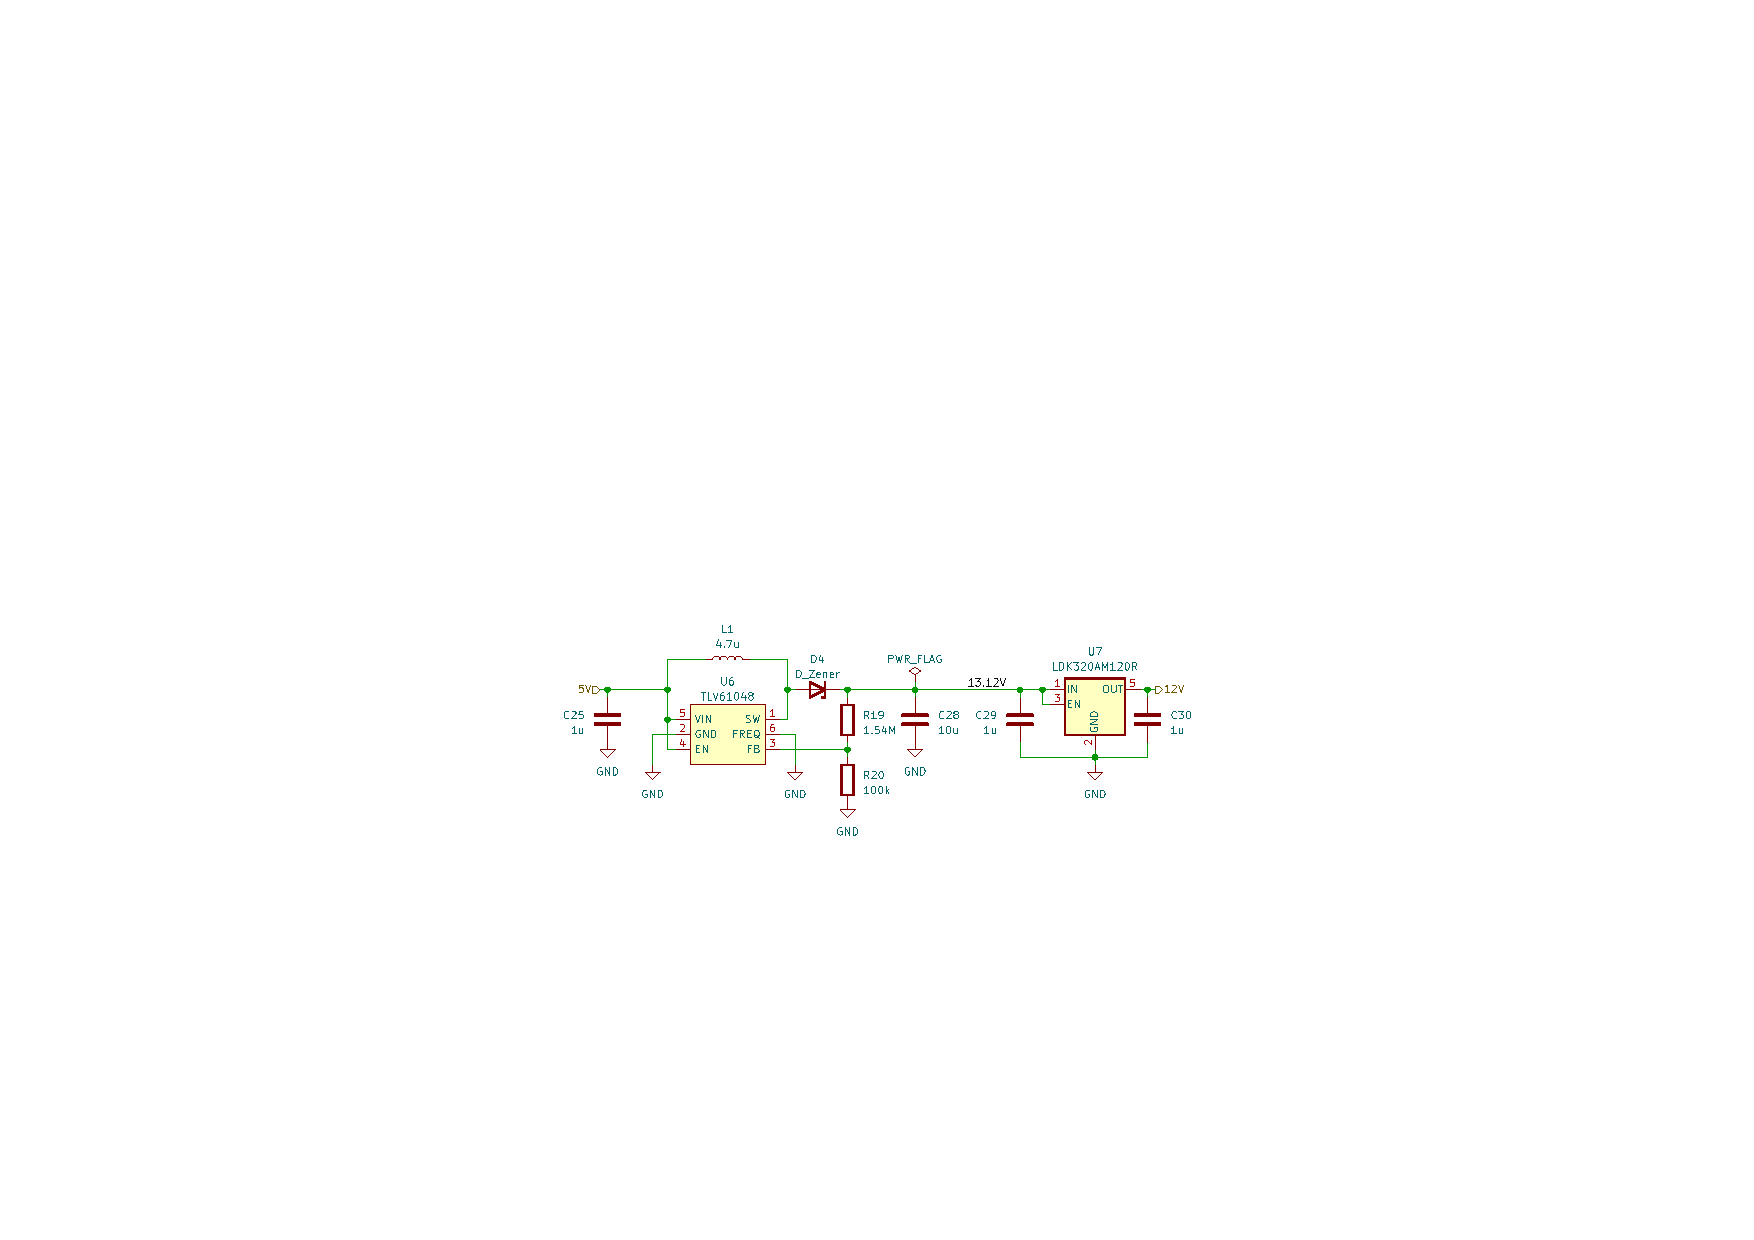
\includegraphics[width=\textwidth]{graphics/power_stage.pdf}
            \caption{Power stage}
      \end{subfigure}
\end{figure}

\subsubsection{Microcontroller and digital domain}

The STM32F205 is a low-end microcontroller with a 120MHz clock speed, 128KB of RAM and the required peripherals needed by the project (DAC, DMA and timers). It was used mainly because it was already stocked in the lab.

The board also features:
\begin{itemize}
      \item An external 25MHz crystal oscillator to drive the microcontroller.
      \item A USB to UART bridge to allow the user to interact with the device via a serial terminal.
      \item An RGBW addressable led used for status indication.
      \item An header connector that exposes the SWD programming interface.
      \item Two buttons: one for reset and one for the BOOT0 pin.
      \item A microsd card slot to store files.
\end{itemize}

\subsection{Software architecture}

The software powering the signal generator board is built upon the \href{https://github.com/NidasioAlberto/miosix-kernel}{Miosix operating system} and features 2 main components:
\begin{itemize}
      \item Drivers for the DAC and DMA peripherals.
      \item A parser built using Flex and Bison that allows to interpret the user input into arbitrary math functions used to generate the output waveform.
\end{itemize}

\subsubsection{Peripherals drivers}

The STM32F205 microcontroller is equipped with a versatile Digital-to-Analog Converter (DAC) peripheral that offers 12-bit resolution and two separate channels, effectively incorporating two DACs. This dual-channel architecture permits simultaneous generation of two distinct analog outputs, allowing our custom board to feature two independent output channels.

\bigbreak

The DAC's conversion process can be initiated through multiple methods. It can be triggered manually via software, which provides direct control over the conversion timing. Alternatively, for applications requiring precise and periodic analog outputs, external triggers can be employed. A common external trigger source is a timer, which can initiate DAC conversions at predetermined intervals, ensuring consistent waveform generation.

\bigbreak

The STM32's DAC is designed also with the capability to generate DMA requests. Once the DAC is ready for new data, it can signal the DMA peripheral to fetch the next data sample. The DMA (Direct Memory Access) controller is a powerful tool designed to handle data transfers independently of the CPU's operation. This peripheral is characterized by sixteen independent streams each of which can be paired with different peripherals, granting a wide range of configuration possibilities. By leveraging the DMA's rapid data transfer capabilities, the DAC can be persistently supplied with data while leaving the CPU time to generate new data samples or perform other tasks.


One of its standout features is the double buffering mode. This mode uses two memory pointers: while one buffer is actively engaged by the DMA stream, the other can be prepared by the CPU, ensuring uninterrupted data flow.

\bigbreak

In the context of the signal generator project, the DMA plays a crucial role. Each DAC is set up to utilize an external trigger originating from a timer. With every trigger event, the DAC issues a DMA request for a new data sample. The DMA has been configured in double buffer mode. Alternatively, a single buffer mode combined with the half-transfer interrupt could have been adopted to achieve a similar result. This integration of the DAC with the DMA and a timer is what ultimately powers the project's ability to generate high-frequency waveforms even with a low end microcontroller such as the STM32F205.

\bigbreak

The developed drivers are C++ classes that abstract the peripherals and allows the programmer to easily configure and use them. In particular the DMA driver is divided into two classes and one struct:
\begin{itemize}
      \item \textbf{DMADriver}: A singleton that manages all DMA streams. When a piece of code needs a stream, it can request it to the DMADriver. If the stream is already in use, the DMADriver will pause the thread until the stream is available, otherwise it will acquire the stream and return it to the caller.
      \item \textbf{DMATransaction}: A struct that holds all configuration parameters for a specific transfer. This includes source and destination addresses, data size, double buffer, interrupts and so on.
      \item \textbf{DMAStream}: This class allows to configure the stream with for a specific transaction, start and stop it and easily handle interrupts. In particular interrupts can be waited with or without a timeout (thank to the Miosix's timed wait feature) or registering a callback function that will be called when the interrupt occurs.
\end{itemize}
